\begin{comment}
\chapter{Sorting}
\end{comment}
\chapter{ソート}

\index{sorting}
\index{ソート}

\begin{comment}
\key{Sorting}
is a fundamental algorithm design problem.
Many efficient algorithms
use sorting as a subroutine,
because it is often easier to process
data if the elements are in a sorted order.

For example, the problem ''does an array contain
two equal elements?'' is easy to solve using sorting.
If the array contains two equal elements,
they will be next to each other after sorting,
so it is easy to find them.
Also, the problem ''what is the most frequent element
in an array?'' can be solved similarly.
\end{comment}

ソート(\key{Sorting})は基本的なアルゴリズム設計の問題である。
データがソート済みだと処理が容易になることはよくあることなので、
多くの効率的なアルゴリズムがソートを内部に含んでいる。

例えば、「数列中に等しい2つの要素があるか?」という問題は、
ソートにより容易に解くことができる。
数列中に2つの同じ要素があるならば、ソート後にそれらは隣接するため
容易に探し出すことができる。
「数列中の最頻値は何か?」という問題も同様に容易に解けるだろう。

\begin{comment}
There are many algorithms for sorting, and they are
also good examples of how to apply
different algorithm design techniques.
The efficient general sorting algorithms
work in $O(n \log n)$ time,
and many algorithms that use sorting
as a subroutine also
have this time complexity.
\end{comment}

ソートには様々なアルゴリズムがあるため、さまざまなアルゴリズム設計のテクニックを
どう適用するか考えるのによい教材となる。
効率的な汎用のソートアルゴリズムの時間計算量は$O(n \log n)$であり、
ソートを内部で利用する多くのアルゴリズムも同様の時間計算量となる。

\begin{comment}
\section{Sorting theory}

The basic problem in sorting is as follows:
\begin{framed}
\noindent
Given an array that contains $n$ elements,
your task is to sort the elements
in increasing order.
\end{framed}
\noindent
For example, the array
\end{comment}

\section{ソートの理論}

ソートの基本的な問題はこのとおりである:
\begin{framed}
\noindent
n要素の数列が与えられたとき、その要素を昇順に並べ替えよ
\end{framed}
\noindent
例えば以下のような数列は:

\begin{center}
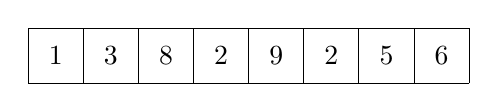
\begin{tikzpicture}[scale=0.7]
\draw (0,0) grid (8,1);
\node at (0.5,0.5) {$1$};
\node at (1.5,0.5) {$3$};
\node at (2.5,0.5) {$8$};
\node at (3.5,0.5) {$2$};
\node at (4.5,0.5) {$9$};
\node at (5.5,0.5) {$2$};
\node at (6.5,0.5) {$5$};
\node at (7.5,0.5) {$6$};
\end{tikzpicture}
\end{center}

\begin{comment}
will be as follows after sorting:
\end{comment}

ソート後以下のようになる:
\begin{center}
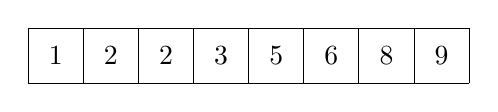
\begin{tikzpicture}[scale=0.7]
\draw (0,0) grid (8,1);
\node at (0.5,0.5) {$1$};
\node at (1.5,0.5) {$2$};
\node at (2.5,0.5) {$2$};
\node at (3.5,0.5) {$3$};
\node at (4.5,0.5) {$5$};
\node at (5.5,0.5) {$6$};
\node at (6.5,0.5) {$8$};
\node at (7.5,0.5) {$9$};
\end{tikzpicture}
\end{center}

\begin{comment}
\subsubsection{$O(n^2)$ algorithms}

\index{bubble sort}

Simple algorithms for sorting an array
work in $O(n^2)$ time.
Such algorithms are short and usually
consist of two nested loops.
A famous $O(n^2)$ time sorting algorithm
is \key{bubble sort} where the elements
''bubble'' in the array according to their values.

Bubble sort consists of $n$ rounds.
On each round, the algorithm iterates through
the elements of the array.
Whenever two consecutive elements are found
that are not in correct order,
the algorithm swaps them.
The algorithm can be implemented as follows:
\end{comment}

\subsubsection{$O(n^2)$ アルゴリズム}

\index{bubble sort}
\index{バブルソート}

数列を並べ替える単純なアルゴリズムは時間計算量$O(n^2)$となる。
そのようなアルゴリズムは短く、通常二重ループで構成される。
有名な時間計算量$O(n^2)$のソートアルゴリズムとしてバブルソート(\key{bubble sort})がある。
これは各要素が値に応じて泡のように数列中を動くことに由来する。

バブルソートは$n$ラウンドの処理で構成される。
このアルゴリズムでは、1回のラウンド毎に数列の要素を1周処理して回る。
もし連続する要素が正しくない、すなわち降順に並んでいる場合、それらを交換する。
実装はこのようになる:
\begin{lstlisting}
for (int i = 0; i < n; i++) {
    for (int j = 0; j < n-1; j++) {
        if (array[j] > array[j+1]) {
            swap(array[j],array[j+1]);
        }
    }
}
\end{lstlisting}

\begin{comment}
After the first round of the algorithm,
the largest element will be in the correct position,
and in general, after $k$ rounds, the $k$ largest
elements will be in the correct positions.
Thus, after $n$ rounds, the whole array
will be sorted.

For example, in the array
\end{comment}

初回のラウンドを終えると、最大の要素は正しい位置、つまり末尾に移動する。
一般的に$k$ラウンド後には上位$k$番目までに大きい要素が正しい位置に移動する。
よって$n$ラウンド後は全要素が正しい位置に移動したことになり、数列全体のソートが完了したことになる。

例えば以下の数列で:

\begin{center}
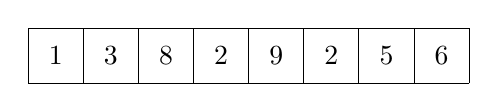
\begin{tikzpicture}[scale=0.7]
\draw (0,0) grid (8,1);

\node at (0.5,0.5) {$1$};
\node at (1.5,0.5) {$3$};
\node at (2.5,0.5) {$8$};
\node at (3.5,0.5) {$2$};
\node at (4.5,0.5) {$9$};
\node at (5.5,0.5) {$2$};
\node at (6.5,0.5) {$5$};
\node at (7.5,0.5) {$6$};
\end{tikzpicture}
\end{center}

\noindent

\begin{comment}
the first round of bubble sort swaps elements
as follows:
\end{comment}

バブルソートの最初のラウンドでは、要素は以下のように交換される:

\begin{center}
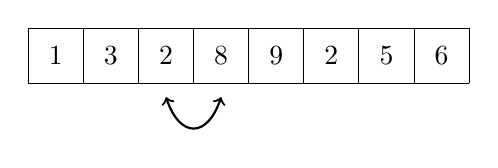
\begin{tikzpicture}[scale=0.7]
\draw (0,0) grid (8,1);
\node at (0.5,0.5) {$1$};
\node at (1.5,0.5) {$3$};
\node at (2.5,0.5) {$2$};
\node at (3.5,0.5) {$8$};
\node at (4.5,0.5) {$9$};
\node at (5.5,0.5) {$2$};
\node at (6.5,0.5) {$5$};
\node at (7.5,0.5) {$6$};

\draw[thick,<->] (3.5,-0.25) .. controls (3.25,-1.00) and (2.75,-1.00) .. (2.5,-0.25);
\end{tikzpicture}
\end{center}

\begin{center}
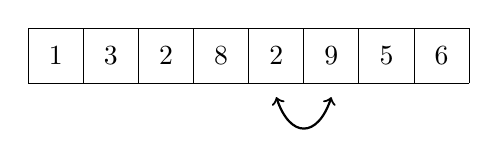
\begin{tikzpicture}[scale=0.7]
\draw (0,0) grid (8,1);
\node at (0.5,0.5) {$1$};
\node at (1.5,0.5) {$3$};
\node at (2.5,0.5) {$2$};
\node at (3.5,0.5) {$8$};
\node at (4.5,0.5) {$2$};
\node at (5.5,0.5) {$9$};
\node at (6.5,0.5) {$5$};
\node at (7.5,0.5) {$6$};

\draw[thick,<->] (5.5,-0.25) .. controls (5.25,-1.00) and (4.75,-1.00) .. (4.5,-0.25);
\end{tikzpicture}
\end{center}

\begin{center}
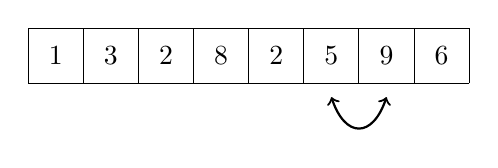
\begin{tikzpicture}[scale=0.7]
\draw (0,0) grid (8,1);
\node at (0.5,0.5) {$1$};
\node at (1.5,0.5) {$3$};
\node at (2.5,0.5) {$2$};
\node at (3.5,0.5) {$8$};
\node at (4.5,0.5) {$2$};
\node at (5.5,0.5) {$5$};
\node at (6.5,0.5) {$9$};
\node at (7.5,0.5) {$6$};

\draw[thick,<->] (6.5,-0.25) .. controls (6.25,-1.00) and (5.75,-1.00) .. (5.5,-0.25);
\end{tikzpicture}
\end{center}

\begin{center}
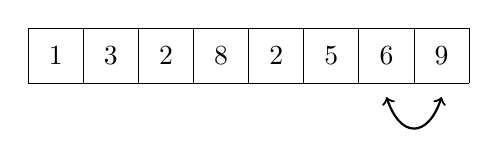
\begin{tikzpicture}[scale=0.7]
\draw (0,0) grid (8,1);
\node at (0.5,0.5) {$1$};
\node at (1.5,0.5) {$3$};
\node at (2.5,0.5) {$2$};
\node at (3.5,0.5) {$8$};
\node at (4.5,0.5) {$2$};
\node at (5.5,0.5) {$5$};
\node at (6.5,0.5) {$6$};
\node at (7.5,0.5) {$9$};

\draw[thick,<->] (7.5,-0.25) .. controls (7.25,-1.00) and (6.75,-1.00) .. (6.5,-0.25);
\end{tikzpicture}
\end{center}

\begin{comment}
\subsubsection{Inversions}

\index{inversion}

Bubble sort is an example of a sorting
algorithm that always swaps \emph{consecutive}
elements in the array.
It turns out that the time complexity
of such an algorithm is \emph{always}
at least $O(n^2)$, because in the worst case,
$O(n^2)$ swaps are required for sorting the array.

A useful concept when analyzing sorting
algorithms is an \key{inversion}:
a pair of array elements
$(\texttt{array}[a],\texttt{array}[b])$ such that
$a<b$ and $\texttt{array}[a]>\texttt{array}[b]$,
i.e., the elements are in the wrong order.
For example, the array
\end{comment}

\subsubsection{転倒}

\index{inversion}
\index{転倒}

バブルソートは、常に数列中で\emph{連続した}要素のみを交換する
アルゴリズムの一例である。
そのようなアルゴリズムの時間計算量は\emph{常に}少なくとも$O(n^2)$となる。
それは最悪ケースではソートに$O(n^2)$回の交換を要するためである。

ソートアルゴリズムの分析に役立つ概念に転倒(\key{inversion})がある。
転倒とは$a<b$でありながら$\texttt{array}[a]>\texttt{array}[b]$となるような
要素の対$(\texttt{array}[a],\texttt{array}[b])$のことである。
つまり、ソート後にあるべき順番に対し誤った順番に並んでいる要素対のことである。
例えば以下の数列:

\begin{center}
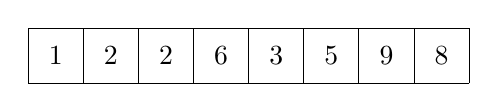
\begin{tikzpicture}[scale=0.7]
\draw (0,0) grid (8,1);
\node at (0.5,0.5) {$1$};
\node at (1.5,0.5) {$2$};
\node at (2.5,0.5) {$2$};
\node at (3.5,0.5) {$6$};
\node at (4.5,0.5) {$3$};
\node at (5.5,0.5) {$5$};
\node at (6.5,0.5) {$9$};
\node at (7.5,0.5) {$8$};
\end{tikzpicture}
\end{center}

\begin{comment}
has three inversions: $(6,3)$, $(6,5)$ and $(9,8)$.
The number of inversions indicates
how much work is needed to sort the array.
An array is completely sorted when
there are no inversions.
On the other hand, if the array elements
are in the reverse order,
the number of inversions is the largest possible:
\[1+2+\cdots+(n-1)=\frac{n(n-1)}{2} = O(n^2)\]

Swapping a pair of consecutive elements that are
in the wrong order removes exactly one inversion
from the array.
Hence, if a sorting algorithm can only
swap consecutive elements, each swap removes
at most one inversion, and the time complexity
of the algorithm is at least $O(n^2)$.
\end{comment}

は3つの転倒$(6,3)$, $(6,5)$, $(9,8)$を含む。
転倒数は数列をソートするためどの程度の作業が必要かを示す。
転倒が一つもない状態がソート完了後の状態と言える。
言い換えると、数列の要素がソート後の逆順に並んでいるとき、
転倒数は最大値:
\[1+2+\cdots+(n-1)=\frac{n(n-1)}{2} = O(n^2)\]
となる。

逆順にならんている連続する2要素の交換は、数列中から
転倒を1つ減らす。
よって、連続する要素のみを交換するソートアルゴリズムでは、
1回の交換で1つの転倒しか減らせないので、
時間計算量は少なくとも$O(n^2)$となる。

\begin{comment}
\subsubsection{$O(n \log n)$ algorithms}

\index{merge sort}

It is possible to sort an array efficiently
in $O(n \log n)$ time using algorithms
that are not limited to swapping consecutive elements.
One such algorithm is \key{merge sort}\footnote{According to \cite{knu983},
merge sort was invented by J. von Neumann in 1945.},
which is based on recursion.
\end{comment}

\subsubsection{$O(n \log n)$アルゴリズム}

\index{merge sort}
\index{マージソート}

交換する要素を連続する要素に限らなければ、より効率よく時間計算量$O(n \log n)$で
数列をソートできる。
その一例がマージソート(\key{merge sort}\footnote{\cite{knu983}によると、
マージソートは1945年にかのJ. von Neumannによって考案された})で、
再帰処理を利用している。

\begin{comment}
Merge sort sorts a subarray \texttt{array}$[a \ldots b]$ as follows:

\begin{enumerate}
\item If $a=b$, do not do anything, because the subarray is already sorted.
\item Calculate the position of the middle element: $k=\lfloor (a+b)/2 \rfloor$.
\item Recursively sort the subarray \texttt{array}$[a \ldots k]$.
\item Recursively sort the subarray \texttt{array}$[k+1 \ldots b]$.
\item \emph{Merge} the sorted subarrays \texttt{array}$[a \ldots k]$ and
\texttt{array}$[k+1 \ldots b]$
into a sorted subarray \texttt{array}$[a \ldots b]$.
\end{enumerate}
\end{comment}

数列の部分列\texttt{array}$[a \ldots b]$のマージソートは、以下のように行う:

\begin{enumerate}
\item もし$a=b$なら部分列はソート済みとみなせるので何もしない。
\item 中央となる位置$k=\lfloor (a+b)/2 \rfloor$を求める。
\item 再帰的に前半部分\texttt{array}$[a \ldots k]$をソートする。
\item 再帰的に後半部分\texttt{array}$[k+1 \ldots b]$をソートする。
\item 2つのソート済み部分列\texttt{array}$[a \ldots k]$と\texttt{array}$[k+1 \ldots b]$を
\emph{マージ}して1つのソート済み部分列\texttt{array}$[a \ldots b]$を作る。
\end{enumerate}

\begin{comment}
Merge sort is an efficient algorithm, because it
halves the size of the subarray at each step.
The recursion consists of $O(\log n)$ levels,
and processing each level takes $O(n)$ time.
Merging the subarrays \texttt{array}$[a \ldots k]$ and \texttt{array}$[k+1 \ldots b]$
is possible in linear time, because they are already sorted.

For example, consider sorting the following array:
\end{comment}

マージソートはステップ毎に対象とする部分列のサイズを半減させていくため、
効率的なアルゴリズムである。
再帰は$O(\log n)$段からなり、各段階の処理は時間計算量で$O(n)$かかる。
部分列\texttt{array}$[a \ldots k]$と\texttt{array}$[k+1 \ldots b]$のマージは、
両部分列がソート済みならば線形時間で終わる。

例として以下の数列のソートを考える:
\begin{center}
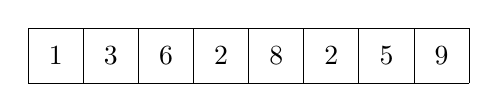
\begin{tikzpicture}[scale=0.7]
\draw (0,0) grid (8,1);
\node at (0.5,0.5) {$1$};
\node at (1.5,0.5) {$3$};
\node at (2.5,0.5) {$6$};
\node at (3.5,0.5) {$2$};
\node at (4.5,0.5) {$8$};
\node at (5.5,0.5) {$2$};
\node at (6.5,0.5) {$5$};
\node at (7.5,0.5) {$9$};
\end{tikzpicture}
\end{center}

\begin{comment}
The array will be divided into two subarrays
as follows:
\end{comment}

この数列は以下のように2つの部分列に分割できる:
\begin{center}
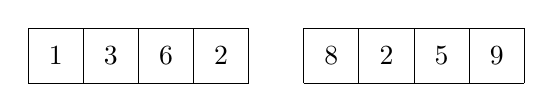
\begin{tikzpicture}[scale=0.7]
\draw (0,0) grid (4,1);
\draw (5,0) grid (9,1);

\node at (0.5,0.5) {$1$};
\node at (1.5,0.5) {$3$};
\node at (2.5,0.5) {$6$};
\node at (3.5,0.5) {$2$};

\node at (5.5,0.5) {$8$};
\node at (6.5,0.5) {$2$};
\node at (7.5,0.5) {$5$};
\node at (8.5,0.5) {$9$};
\end{tikzpicture}
\end{center}

\begin{comment}
Then, the subarrays will be sorted recursively
as follows:
\end{comment}

両部分列は、再帰的にこのようにソートされる:
as follows:
\begin{center}
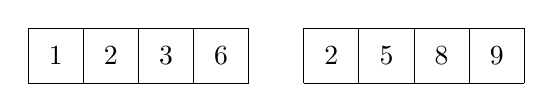
\begin{tikzpicture}[scale=0.7]
\draw (0,0) grid (4,1);
\draw (5,0) grid (9,1);

\node at (0.5,0.5) {$1$};
\node at (1.5,0.5) {$2$};
\node at (2.5,0.5) {$3$};
\node at (3.5,0.5) {$6$};

\node at (5.5,0.5) {$2$};
\node at (6.5,0.5) {$5$};
\node at (7.5,0.5) {$8$};
\node at (8.5,0.5) {$9$};
\end{tikzpicture}
\end{center}

\begin{comment}
Finally, the algorithm merges the sorted
subarrays and creates the final sorted array:
\end{comment}

最終的に、部分列はマージされて最終的に
ソート済み数列が得られる。

\begin{center}
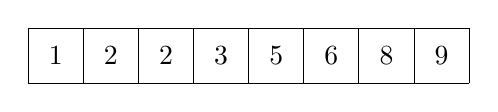
\begin{tikzpicture}[scale=0.7]
\draw (0,0) grid (8,1);
\node at (0.5,0.5) {$1$};
\node at (1.5,0.5) {$2$};
\node at (2.5,0.5) {$2$};
\node at (3.5,0.5) {$3$};
\node at (4.5,0.5) {$5$};
\node at (5.5,0.5) {$6$};
\node at (6.5,0.5) {$8$};
\node at (7.5,0.5) {$9$};
\end{tikzpicture}
\end{center}

\begin{comment}
\subsubsection{Sorting lower bound}

Is it possible to sort an array faster
than in $O(n \log n)$ time?
It turns out that this is \emph{not} possible
when we restrict ourselves to sorting algorithms
that are based on comparing array elements.

The lower bound for the time complexity
can be proved by considering sorting
as a process where each comparison of two elements
gives more information about the contents of the array.
The process creates the following tree:
\end{comment}

\subsubsection{ソートの下限}

時間計算量が$O(n \log n)$よりも小さいソートアルゴリズムは
存在するだろうか?
要素間の大小比較に基づくソートという前提のもとでは、
\emph{不可能}ということがわかっている。

時間計算量の下限は、ソートにおいて2要素の比較から
得られる情報の量について考えると示すことができる。
この手順はこのような木構造に落とすことができる:

\begin{center}
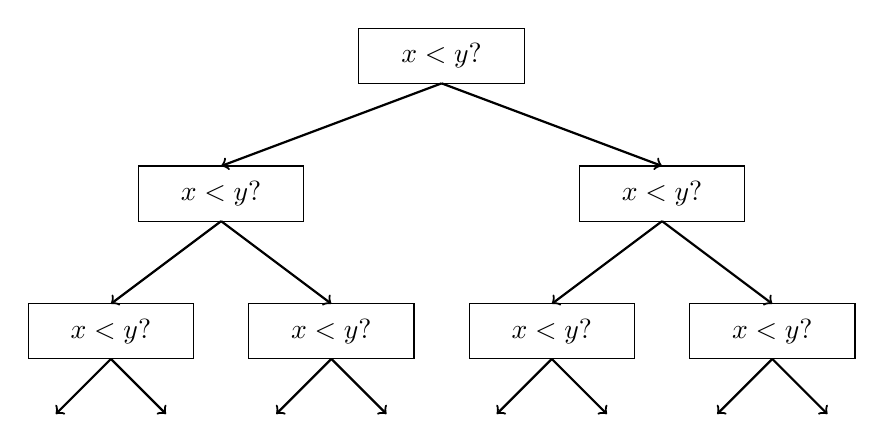
\begin{tikzpicture}[scale=0.7]
\draw (0,0) rectangle (3,1);
\node at (1.5,0.5) {$x < y?$};

\draw[thick,->] (1.5,0) -- (-2.5,-1.5);
\draw[thick,->] (1.5,0) -- (5.5,-1.5);

\draw (-4,-2.5) rectangle (-1,-1.5);
\draw (4,-2.5) rectangle (7,-1.5);
\node at (-2.5,-2) {$x < y?$};
\node at (5.5,-2) {$x < y?$};

\draw[thick,->] (-2.5,-2.5) -- (-4.5,-4);
\draw[thick,->] (-2.5,-2.5) -- (-0.5,-4);
\draw[thick,->] (5.5,-2.5) -- (3.5,-4);
\draw[thick,->] (5.5,-2.5) -- (7.5,-4);

\draw (-6,-5) rectangle (-3,-4);
\draw (-2,-5) rectangle (1,-4);
\draw (2,-5) rectangle (5,-4);
\draw (6,-5) rectangle (9,-4);
\node at (-4.5,-4.5) {$x < y?$};
\node at (-0.5,-4.5) {$x < y?$};
\node at (3.5,-4.5) {$x < y?$};
\node at (7.5,-4.5) {$x < y?$};

\draw[thick,->] (-4.5,-5) -- (-5.5,-6);
\draw[thick,->] (-4.5,-5) -- (-3.5,-6);
\draw[thick,->] (-0.5,-5) -- (0.5,-6);
\draw[thick,->] (-0.5,-5) -- (-1.5,-6);
\draw[thick,->] (3.5,-5) -- (2.5,-6);
\draw[thick,->] (3.5,-5) -- (4.5,-6);
\draw[thick,->] (7.5,-5) -- (6.5,-6);
\draw[thick,->] (7.5,-5) -- (8.5,-6);
\end{tikzpicture}
\end{center}


ここで''$x<y?$''はある2要素$x$と$y$を比較することを示す。
$x<y$であれば手続きは左側、そうでなければ右側に遷移し、
移行手続きが続くものとする。
この手続きの組み合わせは数列の並べ方の数だけあり得るので、
全体で$n!$通り考えられる。
この考えを進めると、木の高さは少なくとも
\[ \log_2(n!) = \log_2(1)+\log_2(2)+\cdots+\log_2(n).\]
必要になる。

右辺の$n$項のうち、後半$n/2$項を$\log_2(n/2)$に置き換えると、
この式の下限がわかる。
この式変形より
\[ \log_2(n!) \ge (n/2) \cdot \log_2(n/2),\]
の関係がわかる。
よって木の高さ、すなわち2要素の最小比較回数が最悪$n \log n$回に
なることがわかる。

\begin{comment}
\subsubsection{Counting sort}

\index{counting sort}

The lower bound $n \log n$ does not apply to
algorithms that do not compare array elements
but use some other information.
An example of such an algorithm is
\key{counting sort} that sorts an array in
$O(n)$ time assuming that every element in the array
is an integer between $0 \ldots c$ and $c=O(n)$.

The algorithm creates a \emph{bookkeeping} array,
whose indices are elements of the original array.
The algorithm iterates through the original array
and calculates how many times each element
appears in the array.
\newpage

For example, the array
\end{comment}

\subsubsection{計数ソート}

\index{counting sort}
\index{計数ソート}

時間計算量の下限$n \log n$は、要素間の比較を用いない
アルゴリズムには適用されない。
その一例が計数ソート(\key{counting sort})である。
このアルゴリズムは数列中の要素が$0 \ldots c$の範囲の整数で、
かつ$c=O(n)$とすると時間計算量が$O(n)$で済む。

このアルゴリズムでは、事前に\emph{カウンタ}配列を作っておく。
この配列のインデックスは元の数列の値に相当する。
このアルゴリズムでは、元の数列の要素を順次見ていき、
各値が何度現れるかを数え上げていく。
\newpage

例えば、以下の数列に対し:
\begin{center}
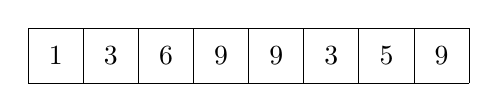
\begin{tikzpicture}[scale=0.7]
\draw (0,0) grid (8,1);
\node at (0.5,0.5) {$1$};
\node at (1.5,0.5) {$3$};
\node at (2.5,0.5) {$6$};
\node at (3.5,0.5) {$9$};
\node at (4.5,0.5) {$9$};
\node at (5.5,0.5) {$3$};
\node at (6.5,0.5) {$5$};
\node at (7.5,0.5) {$9$};
\end{tikzpicture}
\end{center}

\begin{comment}
corresponds to the following bookkeeping array:
\end{comment}

カウンタ配列はこのようになる:
\begin{center}
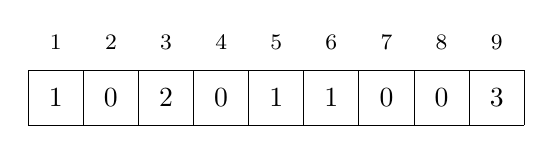
\begin{tikzpicture}[scale=0.7]
\draw (0,0) grid (9,1);
\node at (0.5,0.5) {$1$};
\node at (1.5,0.5) {$0$};
\node at (2.5,0.5) {$2$};
\node at (3.5,0.5) {$0$};
\node at (4.5,0.5) {$1$};
\node at (5.5,0.5) {$1$};
\node at (6.5,0.5) {$0$};
\node at (7.5,0.5) {$0$};
\node at (8.5,0.5) {$3$};

\footnotesize

\node at (0.5,1.5) {$1$};
\node at (1.5,1.5) {$2$};
\node at (2.5,1.5) {$3$};
\node at (3.5,1.5) {$4$};
\node at (4.5,1.5) {$5$};
\node at (5.5,1.5) {$6$};
\node at (6.5,1.5) {$7$};
\node at (7.5,1.5) {$8$};
\node at (8.5,1.5) {$9$};
\end{tikzpicture}
\end{center}

\begin{comment}
For example, the value at position 3
in the bookkeeping array is 2,
because the element 3 appears 2 times
in the original array.

Construction of the bookkeeping array
takes $O(n)$ time. After this, the sorted array
can be created in $O(n)$ time because
the number of occurrences of each element can be retrieved
from the bookkeeping array.
Thus, the total time complexity of counting
sort is $O(n)$.

Counting sort is a very efficient algorithm
but it can only be used when the constant $c$
is small enough, so that the array elements can
be used as indices in the bookkeeping array.
\end{comment}

例えばカウンタ配列の3つめの位置には2が格納されている。
これは元の数列で3が2回登場したことを意味する。

カウンタ配列の構築は$O(n)$時間がかかる。
その後ソート後の配列の構築も、
カウンタ配列の各要素を順次見ていくため$O(n)$時間がかかる。
よって、計数ソートの時間計算量は全体で$O(n)$となる。

計数ソートは非常に効率的だが、元の数列の値を
カウンタ配列のインデックスに用いるため、
$c$が小さいときにしか利用できない。

\begin{comment}
\section{Sorting in C++}

\index{sort@\texttt{sort}}

It is almost never a good idea to use
a home-made sorting algorithm
in a contest, because there are good
implementations available in programming languages.
For example, the C++ standard library contains
the function \texttt{sort} that can be easily used for
sorting arrays and other data structures.

There are many benefits in using a library function.
First, it saves time because there is no need to
implement the function.
Second, the library implementation is
certainly correct and efficient: it is not probable
that a home-made sorting function would be better.
\end{comment}

\section{C++におけるソート}

\index{sort@\texttt{sort}}

ソートアルゴリズムを今から自作することは良い考えではない。
というのも、大抵のプログラミング言語ではよい実装がすでに
利用可能であるためである。
例えばC++標準ライブラリは、数列や他のデータ構造を
容易にソートできる\texttt{sort}関数を提供している。

このライブラリ関数を用いることには色々な利点がある。
まず、自分で実装しなくてよいので時間を節約できる。
また、ライブラリの実装は自作の関数ではそうそう超えられない程度まで
正確かつ効率的に作られている。

\begin{comment}
In this section we will see how to use the
C++ \texttt{sort} function.
The following code sorts
a vector in increasing order:
\begin{lstlisting}
vector<int> v = {4,2,5,3,5,8,3};
sort(v.begin(),v.end());
\end{lstlisting}
After the sorting, the contents of the
vector will be
$[2,3,3,4,5,5,8]$.
The default sorting order is increasing,
but a reverse order is possible as follows:
\begin{lstlisting}
sort(v.rbegin(),v.rend());
\end{lstlisting}
An ordinary array can be sorted as follows:
\begin{lstlisting}
int n = 7; // array size
int a[] = {4,2,5,3,5,8,3};
sort(a,a+n);
\end{lstlisting}
\newpage
\end{comment}

この項では、C++の\texttt{sort}関数についてみていこう。
以下のコードはvectorを昇順にソートする:
\begin{lstlisting}
vector<int> v = {4,2,5,3,5,8,3};
sort(v.begin(),v.end());
\end{lstlisting}
ソート後のvectorの中身は以下のとおりである:
$[2,3,3,4,5,5,8]$.
デフォルトのソート順序は昇順である。
しかしこのようにすれば逆順にできる:
\begin{lstlisting}
sort(v.rbegin(),v.rend());
\end{lstlisting}
通常の配列は以下のようになる:
\begin{lstlisting}
int n = 7; // array size
int a[] = {4,2,5,3,5,8,3};
sort(a,a+n);
\end{lstlisting}
\newpage

\begin{comment}
The following code sorts the string \texttt{s}:
\begin{lstlisting}
string s = "monkey";
sort(s.begin(), s.end());
\end{lstlisting}
Sorting a string means that the characters
of the string are sorted.
For example, the string ''monkey'' becomes ''ekmnoy''.
\end{comment}

以下のコードは文字列\texttt{s}をソートする:
\begin{lstlisting}
string s = "monkey";
sort(s.begin(), s.end());
\end{lstlisting}
文字列をソートすると、文字列中の文字をソートしたものが得られる。
例えば文字列''monkey''をソートすると''ekmnoy''が得られる。

\begin{comment}
\subsubsection{Comparison operators}

\index{comparison operator}

The function \texttt{sort} requires that
a \key{comparison operator} is defined for the data type
of the elements to be sorted.
When sorting, this operator will be used
whenever it is necessary to find out the order of two elements.

Most C++ data types have a built-in comparison operator,
and elements of those types can be sorted automatically.
For example, numbers are sorted according to their values
and strings are sorted in alphabetical order.
\end{comment}

\subsubsection{比較演算子}

\index{comparison operator}
\index{比較演算子}

\texttt{sort}関数は、ソート対象の配列の要素のデータ型が
比較演算子(\key{comparison operator})を持つことを要求する。
ソート過程で、この演算子は2つの要素のどちらを前にすべきか
決定するのに用いる。

大抵のC++のデータ型は組み込みの比較演算子を持つので、
これらを要素とする配列は自動的にソート可能である。
例えば数値型は値、文字列型はアルファベット順でソートされる。

\index{pair@\texttt{pair}}

\begin{comment}

Pairs (\texttt{pair}) are sorted primarily according to their
first elements (\texttt{first}).
However, if the first elements of two pairs are equal,
they are sorted according to their second elements (\texttt{second}):
\begin{lstlisting}
vector<pair<int,int>> v;
v.push_back({1,5});
v.push_back({2,3});
v.push_back({1,2});
sort(v.begin(), v.end());
\end{lstlisting}
After this, the order of the pairs is
$(1,2)$, $(1,5)$ and $(2,3)$.
\end{comment}


ペア型(\texttt{pair})は、1つめの要素(\texttt{first})でソートされる。
しかし、もし2つのペアにおいて1つめの要素が等しい場合、
続いて2つ目の要素(\texttt{second})によってソートされる:
\begin{lstlisting}
vector<pair<int,int>> v;
v.push_back({1,5});
v.push_back({2,3});
v.push_back({1,2});
sort(v.begin(), v.end());
\end{lstlisting}
上記vectorは、ソート後$(1,2)$, $(1,5)$, $(2,3)$の順になる。


\index{tuple@\texttt{tuple}}

\begin{comment}
In a similar way, tuples (\texttt{tuple})
are sorted primarily by the first element,
secondarily by the second element, etc.\footnote{Note that in some older compilers,
the function \texttt{make\_tuple} has to be used to create a tuple instead of
braces (for example, \texttt{make\_tuple(2,1,4)} instead of \texttt{\{2,1,4\}}).}:
\begin{lstlisting}
vector<tuple<int,int,int>> v;
v.push_back({2,1,4});
v.push_back({1,5,3});
v.push_back({2,1,3});
sort(v.begin(), v.end());
\end{lstlisting}
After this, the order of the tuples is
$(1,5,3)$, $(2,1,3)$ and $(2,1,4)$.
\end{comment}

同様に、タプル型(\texttt{tuple})もまずは先頭要素でソートされる。
先頭要素同士が等しい場合、次に2番目の要素、以下同様に処理される
\footnote{一部の古いコンパイラでは、タプルの生成に中括弧ではなく
\texttt{make\_tuple}関数を要する。
例えば\texttt{\{2,1,4\}}の代わりに\texttt{make\_tuple(2,1,4)}としなければならない。}
\begin{lstlisting}
vector<tuple<int,int,int>> v;
v.push_back({2,1,4});
v.push_back({1,5,3});
v.push_back({2,1,3});
sort(v.begin(), v.end());
\end{lstlisting}
上記vectorはソート後$(1,5,3)$, $(2,1,3)$, $(2,1,4)$の順となる。

\begin{comment}
\subsubsection{User-defined structs}

User-defined structs do not have a comparison
operator automatically.
The operator should be defined inside
the struct as a function
\texttt{operator<},
whose parameter is another element of the same type.
The operator should return \texttt{true}
if the element is smaller than the parameter,
and \texttt{false} otherwise.

For example, the following struct \texttt{P}
contains the x and y coordinates of a point.
The comparison operator is defined so that
the points are sorted primarily by the x coordinate
and secondarily by the y coordinate.
\end{comment}

\subsubsection{ユーザー定義構造体}

ユーザー定義の構造体には自動で比較演算子が定義されない。
比較演算子は\texttt{operator<}として構造体内で定義されなければならない。
この演算子は引数に同じ型のもう片方の要素をとり、
呼び出し元要素が引数側の要素より小さいなら\texttt{true}、
そうでなければ\texttt{false}を返すようにする。

例えば頂点のx,y座標を格納する\texttt{P}という型を作成したとする。
この型の比較演算子として、例えばまずx座標で大小比較し、
x座標が等しいなら次にy座標で
大小比較するという定義が考えられる。

\begin{lstlisting}
struct P {
    int x, y;
    bool operator<(const P &p) {
        if (x != p.x) return x < p.x;
        else return y < p.y;
    }
};
\end{lstlisting}

\begin{comment}
\subsubsection{Comparison functions}

\index{comparison function}

It is also possible to give an external
\key{comparison function} to the \texttt{sort} function
as a callback function.
For example, the following comparison function \texttt{comp}
sorts strings primarily by length and secondarily
by alphabetical order:
\end{comment}


\subsubsection{比較関数}

\index{comparison function}
\index{比較関数}

\texttt{sort}関数は、外部からコールバック関数として比較関数(\key{comparison function})
を渡すことができる。
例えば以下のような比較関数\texttt{comp}を使うと、
文字列をまつ長さでソートし、同着なら次に辞書順で比較する
といいうようなソートができる:

\begin{lstlisting}
bool comp(string a, string b) {
    if (a.size() != b.size()) return a.size() < b.size();
    return a < b;
}
\end{lstlisting}
\begin{comment}
Now a vector of strings can be sorted as follows:
\end{comment}
文字列型のvectorはこのようにソートされる:
\begin{lstlisting}
sort(v.begin(), v.end(), comp);
\end{lstlisting}

\begin{comment}
\section{Binary search}

\index{binary search}

A general method for searching for an element
in an array is to use a \texttt{for} loop
that iterates through the elements of the array.
For example, the following code searches for
an element $x$ in an array:
\end{comment}

\section{二分探索}

\index{binary search}
\index{二分探索}

数列中で要素を探す一般的な方法として、
全要素を\texttt{for}ループで順次処理していく方法がある。
例えばこのコードは数列中から要素$x$を探す。

\begin{lstlisting}
for (int i = 0; i < n; i++) {
    if (array[i] == x) {
        // x found at index i
    }
}
\end{lstlisting}


\begin{comment}
The time complexity of this approach is $O(n)$,
because in the worst case, it is necessary to check
all elements of the array.
If the order of the elements is arbitrary,
this is also the best possible approach, because
there is no additional information available where
in the array we should search for the element $x$.

However, if the array is \emph{sorted},
the situation is different.
In this case it is possible to perform the
search much faster, because the order of the
elements in the array guides the search.
The following \key{binary search} algorithm
efficiently searches for an element in a sorted array
in $O(\log n)$ time.
\end{comment}

\begin{comment}
このアプローチは最悪ケースでは数列の全要素をチェックするので、
時間計算量は$O(n)$となる。
数列の要素の並びに特徴がなく、他の追加情報がないという前提では、
要素$x$を探すのにこれは最良のアプローチである。

しかし、数列が\emph{ソート済み}である場合、事情が異なる。
その場合、検索過程で要素の並びにより追加情報を得られるため、
検索を高速化できる。
以下の二分探索(\key{binary search)アルゴリズムは、
ソート済み配列からデータを$O(\log n)$で効率的に検索できる。
\end{comment}

\begin{comment}
\subsubsection{Method 1}

The usual way to implement binary search
resembles looking for a word in a dictionary.
The search maintains an active region in the array,
which initially contains all array elements.
Then, a number of steps is performed,
each of which halves the size of the region.

At each step, the search checks the middle element
of the active region.
If the middle element is the target element,
the search terminates.
Otherwise, the search recursively continues
to the left or right half of the region,
depending on the value of the middle element.

The above idea can be implemented as follows:

\begin{lstlisting}
int a = 0, b = n-1;
while (a <= b) {
    int k = (a+b)/2;
    if (array[k] == x) {
        // x found at index k
    }
    if (array[k] > x) b = k-1;
    else a = k+1;
}
\end{lstlisting}
\end{comment}

\subsubsection{方法1}

二分探索を実装する一般的な方法は、辞書から単語を探す手順を
真似ればよい。
探索過程では、配列中で探索対象の領域を絞り込んでいく。
この探索対象領域は初期状態では配列全体となるが、1ステップごとに
半分の大きさにしていく。

各ステップでは、探索対象領域の中央の要素をチェックする。
もし中央の要素が検索値と一致するなら探索は終了する。
そうでなければ、中央の要素と検索値の大小に応じて、
探索対象を中央要素の手前か後いずれか半分として
再帰的に探索を行う。

このアイデアを実装するとこのようになる:

\begin{lstlisting}
int a = 0, b = n-1;
while (a <= b) {
    int k = (a+b)/2;
    if (array[k] == x) {
        // k番目の要素がxであることを見つけた
    }
    if (array[k] > x) b = k-1;
    else a = k+1;
}
\end{lstlisting}

\begin{comment}
In this implementation, the active region is $a \ldots b$,
and initially the region is $0 \ldots n-1$.
The algorithm halves the size of the region at each step,
so the time complexity is $O(\log n)$.
\end{comment}

この実装では探索対象の領域は$a \ldots b$で表され、
初期状態ではその領域は$0 \ldots n-1$である。
このアルゴリズムはステップ毎に領域を半分にしていくので、
時間計算量は$O(\log n)$である。

\begin{comment}
\subsubsection{Method 2}

An alternative method to implement binary search
is based on an efficient way to iterate through
the elements of the array.
The idea is to make jumps and slow the speed
when we get closer to the target element.

The search goes through the array from left to
right, and the initial jump length is $n/2$.
At each step, the jump length will be halved:
first $n/4$, then $n/8$, $n/16$, etc., until
finally the length is 1.
After the jumps, either the target element has
been found or we know that it does not appear in the array.

The following code implements the above idea:
\begin{lstlisting}
int k = 0;
for (int b = n/2; b >= 1; b /= 2) {
    while (k+b < n && array[k+b] <= x) k += b;
}
if (array[k] == x) {
    // x found at index k
}
\end{lstlisting}
\end{comment}

\subsubsection{方法2}

二分探索の別の実装法としては、効率的に配列を
辿っていく手段が使える。
アイデアとしては、最初は大きく要素間をジャンプしていき、
検索値に近づくに従いジャンプの距離をだんだん短くしていく
ことになる。

この探索では、配列の先頭から末尾まで要素を辿っていく。
初回のジャンプ距離は$n/2$とする。
ステップ毎にジャンプ距離は$n/4$, $n/8$, $n/16$と半減していき、
最終的には1となる。
ジャンプの度に検索値が見つかるか、もしくは検索値を飛び越してしまい
これ以上あとには現れないかを判定していく。

このアイデアを実装するとこのようになる:
\begin{lstlisting}
int k = 0;
for (int b = n/2; b >= 1; b /= 2) {
    while (k+b < n && array[k+b] <= x) k += b;
}
if (array[k] == x) {
    // k番目の要素がxであることを見つけた
}
\end{lstlisting}

\begin{comment}
During the search, the variable $b$
contains the current jump length.
The time complexity of the algorithm is $O(\log n)$,
because the code in the \texttt{while} loop
is performed at most twice for each jump length.
\end{comment}

この探索において、変数$b$は現在のジャンプ距離を示す。
このコード中、\texttt{while}ループは各ジャンプ距離に対し
高々2回しか実行されないので、このアルゴリズムの
時間計算量は$O(\log n)$である。

\begin{comment}
\subsubsection{C++ functions}

The C++ standard library contains the following functions
that are based on binary search and work in logarithmic time:

\begin{itemize}
\item \texttt{lower\_bound} returns a pointer to the
first array element whose value is at least $x$.
\item \texttt{upper\_bound} returns a pointer to the
first array element whose value is larger than $x$.
\item \texttt{equal\_range} returns both above pointers.
\end{itemize}
\end{comment}

\subsubsection{C++の関数}

C++の標準ライブラリは、二分探索を用いて対数時間で探索を終える
関数を持つ:

\begin{itemize}
\item \texttt{lower\_bound} は配列中で値が少なくとも$x$である
最小の要素へのイテレータを返す。
\item \texttt{upper\_bound} は配列中で値が$x$を超える
最小の要素へのイテレータを返す。
\item \texttt{equal\_range}は上記両方のイテレータを返す。.
\end{itemize}

\begin{comment}
The functions assume that the array is sorted.
If there is no such element, the pointer points to
the element after the last array element.
For example, the following code finds out whether
an array contains an element with value $x$:

\begin{lstlisting}
auto k = lower_bound(array,array+n,x)-array;
if (k < n && array[k] == x) {
    // x found at index k
}
\end{lstlisting}

Then, the following code counts the number of elements
whose value is $x$:

\end{comment}

これらの関数は配列がソート済みであることを前提とする。
条件を満たす要素が見つからない場合、
これらの関数は配列の末尾へのイテレータを返す。
例えば、このコードは配列中に$x$ちょうどの値を
持つかどうかを示す。

\begin{lstlisting}
auto k = lower_bound(array,array+n,x)-array;
if (k < n && array[k] == x) {
    // k番目の要素がxであることを見つけた
}
\end{lstlisting}

以下のコードは、配列中$x$の出現回数を出力する:

\begin{lstlisting}
auto a = lower_bound(array, array+n, x);
auto b = upper_bound(array, array+n, x);
cout << b-a << "\n";
\end{lstlisting}

\begin{comment}
Using \texttt{equal\_range}, the code becomes shorter:
\end{comment}

\texttt{equal\_range}を使えばさらに短く書くことができる:

\begin{lstlisting}
auto r = equal_range(array, array+n, x);
cout << r.second-r.first << "\n";
\end{lstlisting}


\begin{comment}
\subsubsection{Finding the smallest solution}

An important use for binary search is
to find the position where the value of a \emph{function} changes.
Suppose that we wish to find the smallest value $k$
that is a valid solution for a problem.
We are given a function $\texttt{ok}(x)$
that returns \texttt{true} if $x$ is a valid solution
and \texttt{false} otherwise.
In addition, we know that $\texttt{ok}(x)$ is \texttt{false}
when $x<k$ and \texttt{true} when $x \ge k$.
The situation looks as follows:
\end{comment}

\subsubsection{最小値の探索}

二分探索の重要な応用として、ある\emph{関数}の値が変化する
位置の探索がある。
例えば条件を満たす最小の値$k$を求める問題を考えよう。
関数$\texttt{ok}(x)$が与えられたとする。
この関数は$x$が条件を満たすなら\texttt{true}、そうでなければ
\texttt{false}を返す。
ここでは、$\texttt{ok}(x)$は$x<k$のとき\texttt{false}、
$x \ge k$のとき\texttt{true}を返すようなものであることが
わかっているとする。
この状況をわかりやすく表すとこのようになる:

\begin{center}
\begin{tabular}{r|rrrrrrrr}
$x$ & 0 & 1 & $\cdots$ & $k-1$ & $k$ & $k+1$ & $\cdots$ \\
\hline
$\texttt{ok}(x)$ & \texttt{false} & \texttt{false}
& $\cdots$ & \texttt{false} & \texttt{true} & \texttt{true} & $\cdots$ \\
\end{tabular}
\end{center}

\noindent
\begin{comment}
Now, the value of $k$ can be found using binary search:
\end{comment}

この時、値$k$は二分探索で求められる:

\begin{lstlisting}
int x = -1;
for (int b = z; b >= 1; b /= 2) {
    while (!ok(x+b)) x += b;
}
int k = x+1;
\end{lstlisting}

\begin{comment}
The search finds the largest value of $x$ for which
$\texttt{ok}(x)$ is \texttt{false}.
Thus, the next value $k=x+1$
is the smallest possible value for which
$\texttt{ok}(k)$ is \texttt{true}.
The initial jump length $z$ has to be
large enough, for example some value
for which we know beforehand that $\texttt{ok}(z)$ is \texttt{true}.

The algorithm calls the function \texttt{ok}
$O(\log z)$ times, so the total time complexity
depends on the function \texttt{ok}.
For example, if the function works in $O(n)$ time,
\end{comment}

この探索では、$\texttt{ok}(x)$が\texttt{false}となる最大の$x$を求めている。
そのため、次の値$k=x+1$は$\texttt{ok}(k)$が\texttt{true}となる最小の値となる。
初期ジャンプ距離$z$は、 $\texttt{ok}(z)$が明らかに\texttt{true}となるのに
十分な値にする帆必要がある。

このアルゴリズムは関数\texttt{ok}を$O(\log z)$回呼び出すので、
時間計算量は関数\texttt{ok}に依存する。
例えばこの関数が時間計算量$O(n)$であれば、
この探索全体の時間計算量は$O(n \log z)$となる。

\begin{comment}
\subsubsection{Finding the maximum value}

Binary search can also be used to find
the maximum value for a function that is
first increasing and then decreasing.
Our task is to find a position $k$ such that
\end{comment}

\subsubsection{最大値の探索}

二分探索は、上に凸である(入力に応じて最初増加し、その後減少する)ような
関数における最大値の探索にも応用可能である。
以下の条件を満たす$k$を求める問題を考えよう:

\begin{itemize}
\item
$f(x)<f(x+1)$ when $x<k$, and
\item
$f(x)>f(x+1)$ when $x \ge k$.
\end{itemize}

\begin{comment}
The idea is to use binary search
for finding the largest value of $x$
for which $f(x)<f(x+1)$.
This implies that $k=x+1$
because $f(x+1)>f(x+2)$.
The following code implements the search: 
\end{comment}

アイデアとしては、$f(x)<f(x+1)$を満たす最大の$x$を
二分探索で求めることである。
そのような$x$に対し$f(x+1)>f(x+2)$となるため
$k=x+1$が求める値となる。
このアイデアは以下のように実装できる:

\begin{lstlisting}
int x = -1;
for (int b = z; b >= 1; b /= 2) {
    while (f(x+b) < f(x+b+1)) x += b;
}
int k = x+1;
\end{lstlisting}

\begin{comment}
Note that unlike in the ordinary binary search,
here it is not allowed that consecutive values
of the function are equal.
In this case it would not be possible to know
how to continue the search.
\end{comment}

通常の二分探索と異なり、ここでは関数中で連続した入力値に対し
同じ値が返るケースを考慮していない。
そのような場合、探索を続けることができない。
